%
% File: chap01.tex
% Author: Victor F. Brena-Medina
% Description: Introduction chapter where the biology goes.
%
\let\textcircled=\pgftextcircled
\chapter{Introduccion}
\label{chap:intro}

\initial{P}ara esta primera parte se presentara la problematica en el tema de seguridad en ambientes web, las soluciones que se han aplicado y las herramientas que se usan para detectar vulnerabilidades de seguridad.

%=======
\section{Entorno Actual}
\label{sec:sec01}

Actualmente $1/3$ del GDP Mundial esta concentrado en la web, sitios de comercio como Amazon.com, Ebay.com y Alibaba.com entre otros dominan el mercado comercial como nunca antes, los bancos han agilizado sus servicios atraves de apliaciones web y desde pequenos hasta grandes negocios son beneficiados por el uso de sistemas de informacion para aumentar su productividad.

Con el aumento de la integracion de la web en nuestra vida cotidiana, en igual proporcion a subido los ataques a estos sistemas. El resguardo de la informacion, privacidad como tambien  protejerse de atacantes es una de los problemas mas grandes en servicios web en la actualidad. Asegurar que las aplicaciones web sean lo mas seguras posibles sea a convertido en una necesidad y esta dejando de ser un caracteristica atractiva de una aplicacion.

Una de las formas de resguardar las aplicaciones es atraves de un proceso de pruebas, denominado penetration testing o Pentest. Este proceso de pruebas implica correr softwares de reconocimiento para obtener informacion de el objetivo, usar esta informacion para detectar fallas dentro de la aplicacion o por la periferia, para luego encontrar alguna vulnerabilidad que permita ingresar al sistema.

Existen varias metodologias para un buen pentest. \cite{OWASP}

\begin{enumerate}
\item{OWASP testing guide}
\item{PCI Penetration testing guide}
\item{Penetration Testing Execution Standard}
\item{NIST 800-115}
\item{Penetration Testing Framework}
\item{Information Systems Security Assessment Framework (ISSAF)}
\item{Open Source Security Testing Methodology Manual (“OSSTMM”)}
\end{enumerate}

\section{Metodologias}

Para poder conducir un pentest optimo, se debe recordar las cinco fases de analisis y recopilamiento de informacion. Resumidas a continuacion.

\begin{enumerate}
\item{Footprinting}
\item{Scanning}
\item{Exploit}
\item{Payload}
\item{Persitence}
\end{enumerate}

\subsection{Footprinting}
La fase de footprinting consiste en buscar informacion publica de el objetivo a analisar, cuentas de linkedin, facebook, twitter, registros publics gubernamentales etc. Toda la informacion recopilada en esta fase puede ser muy valiosa en el futuro.

\subsection{Scanning}
La fase de escanear consiste en correr port scanners como Nmap para intentar enumarar las infraestrutura del objetivo, puertos publicos o privados, e intentar ver que servicios se albergan detras de estos junto con la version de ese software. Esta informacion es muy importante al momento de querer correr algun exploit sobre el objetivo.

\subsection{Exploit}
La fase de exploit consiste en analizar los datos recopilados en las dos fases anteriores e intentar encontrar una falla o vulnerabilidad que permita la ejecucion de codigo o extraccion de informacion no autorizada. Tambien es posible que al tener las versiones y servicios de los endpoints, encontrar una vulnerabrZilidad ya reportarda y que el objetivo no a actualizado.

\subsection{Payload}

La fase de payload consiste en que una vez encontrada la falla de seguridad o vulnerabilidad, usarla para conseguir acceso al sistema, y subir un script o un programa que ejecute el ataque deseado, dentros de estos ataques existen scripts malisios, malware, shells reversos etc.

\subsection{Persistence}

La fase de persistencia consiste en que una vez que se haya ejecutado el payload se debe instaurar una forma de acceso a la maquina sin pasar por la vulnerabilidad encontrada, mas bien levantar servicios o conectarse a servidores externos controlados por el atacante que permitan el facil acceso a la maquina atacada en caso de que la vulnerabilidad sea arreglada.



\section{Herramientas}

Para poder ejecutar un pentest eficiente es necesario el uso de herramientas que agilizen el proceso de obtencion de datos y colaboren en encontrar vulnerabilidades dentro de cualquier ambiente y aplicacion. A continuacion se presentara una coleccion de herramientas estandar en la industria de seguridad en informatica.

\subsection{Scanners}

\subsubsection{Vulnerabilidad}

\begin{enumerate}
\item{Nessus [Multi]} \\
Nesus es un no de los scanners de vulnerabilidades mas usados por auditores y analistas de seguridad en el mundo, los usuarios pueden correr multiples scans, crear politicas de seguridad, generar scans por horario y generacion de reportes via email. Tambien integra con una gran mayoria de productos de seguridad y hardware usado por profesionales. 

Permite el analisis en ambientes virtualizados y plataformas en la nube, como tambien deteccion de malware y el uso de botnets.

\item{OpenVAS [Win, Unix]}

El Open Vulnerability Assessment System (OpenVAS) es un framework compuesto de varios servicios y herramientas que ofrecen una comprensiva y poderosa plataforma de escanear y manejo de vulnerabilidades.

El escaner esta acompanado por un constante flujo de mejoras de la NVT (Network Vulnerability Tests) con un total de 47.000 para Junio, 2016.

\item{Core Impact [Win]}
Core impact no es barato, pero es considerado ampliamente como la herramienta de explotación mas potente en la actualidad. Contiene una gran base de datos de exploits profesionales, tambien tiene mecanismos como hacer pivotes entre maquinas infectadas atraves de tuneles encriptados. 

\item{Nexpose [Win,Unix]}


\end{enumerate}

\subsubsection{Web}

\begin{enumerate}
\item{Burp Suite [Multi]}
Burp Suite es un servidor proxy que permite la captura y forward de paquetes para poder hacer crawling sobre una pagina para poder mapearla 
\item{Nikto [Multi]}
\item{w3af [Multi]}
\item{WebScarab [Multi]}
\item{sqlmap [Multi]}
Permite correr conocidos strings de sql que permiten analizar si existen vulnerabilidades del tipo sql injection, su fuerte es blind sql injection pero permite tambien in-band sql injection y out-of-band.
\item{skipfish [Multi]}
\item{Acunetix WVS [Multi]}
\item{AppScan [Multi]}

\end{enumerate}

\subsection{Sniffers}
\begin{enumerate}
\item{Wireshark [Multi]}
Analizador de datos en la capa de red, permite la captura de paquetes y analisis de headers y metadata en un flujo de datos.
\item{Cain and Abel [Win] }
\item{Tcpdump [Multi] }
\item{Ettercap [Multi] }
Herramienta que permite montar ataques MitM (Man in the Middle) quedo descontinuada una vez que SSL se hizo mas popular e implementado a nivel global. Ultimamente ataques que permiten descarcatar el certificado SSL, a convertido a esta herramienta util nuevamente.
\item{NetStumbler [Win] }
\item{dsniff [Multi] }
\item{NetworkMiner [Win] }
\end{enumerate}

\subsection{Exploitation}

\begin{enumerate}
\item{Metasploit [Multi]}
Framework de exploits y payloads que permite el facil manejo de estas. Conocido como uno de los mejores frameworks del mundo para penetration testing. Permite generacion de scripts y persistencia atraves de pivots y herramientas propias del framework como Rail Gun.
\item{w3af [Multi] }
\item{Core Impact [Win] }
\item{Social Engineer Toolkit [Multi] }
\item{BeEF [Multi]}
\end{enumerate}

\subsection{Crackers}

\begin{enumerate}
\item{Aircrack-ngp [Unix]}
El suite de Aircrack permite el analisis de redes Wifi en la banda 2.4 para atacar el estandar 802.11, esta herramienta permite escanear el aire por redes en el vecindario, captura e injeccion de paquetes, levantar access points falsos y crackear passwords de la red.
\item{Cain and Abel [Win]}
\item{John the Ripper [Multi]}
John es la herramienta open source mas popular para crackear passwords a traves de fuerza bruta, permite generacion de diccionarios para atacar como tambien reemplazos por patron para aumentar aun mas el espectro de cobertura por los diccionarios.
\item{THC Hydra [Unix]}
Hydra es otro password cracker que recibe su nombre por su capacidad de generar threads para acelerar el proceso de fuerza bruta hacia servicios (1 cabeza de la hydra = un hilo de procesamiento). Permite ataques hacia servidores ssh, ftp, http, smtp entre otros.
\item{ophcrack [Multi]}
\item{Medusa [Unix]}


\end{enumerate}

\section{System Specifications}

All programs and builds will be done under my own personal computer which is an ASUS ZenBook UX305, Processor Intel Core \texttrademark


% \label{subsec:subsec01}

% Begins a subsection.

% %A figures matrix.
% \begin{figure}[t!]
% \centering
% \begin{minipage}{3.3cm}
%     \centering
%     \subtop[]{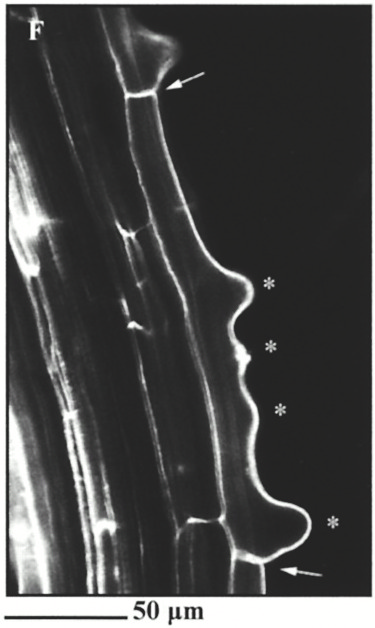
\includegraphics[height=0.28\textheight]{fig01/Nswellings}\label{sf:multiRH02a}}
% \end{minipage}
% \hspace{0.5cm}
% \begin{minipage}{3.3cm}
%     \centering
%     \subtop[]{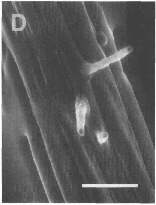
\includegraphics[height=0.27\textheight]{fig01/Mswellings}\label{sf:multiRH02b}}
% \end{minipage}
% \hspace{1.3cm}
% \begin{minipage}{3.3cm}
%     \centering
%     \subtop[]{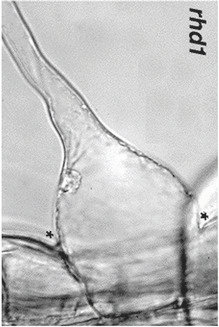
\includegraphics[height=0.27\textheight]{fig01/rhd1}\label{sf:multiRH02c}}
% \end{minipage}
% \\ \vspace{0.1cm}
% \begin{minipage}{10cm}
%     \centering
%     \subtop[]{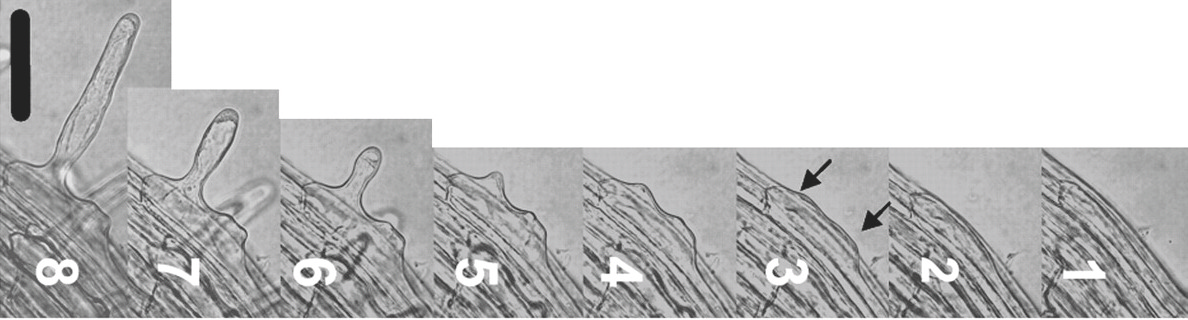
\includegraphics[height=0.145\textheight]{fig01/mutantrhd6}\label{sf:multiRH02d}}
% \end{minipage}
% \\ \vspace{0.1cm}
% \begin{minipage}{10cm}
%     \centering
%     \subtop[]{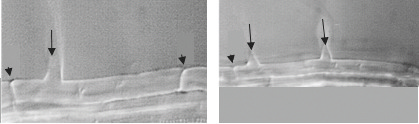
\includegraphics[height=0.16\textheight]{fig01/auxab}\label{sf:multiRH02e}}
% \end{minipage}
% \mycaption[Hair-forming mutant cells.]{(a) A mutant RH cell. Asterisks show multiple sites of RH initiation in a single root hair cell (indicated by the arrows). Figure reproduced from \cite{rigas01}. (b)~Hair-forming cell with three RH initiation locations. The bar represents $50\mu m$. Figure reproduced from \cite{massuci01}. (c) Large bump in mutant {\itshape rhd1}. Figure reproduced from \cite{griersonRH}. (d) Mutant overexpressing gene {\itshape ROP2}; from right-hand to left-hand, numbers indicate progressive snapshots at different times. RH initiation sites are indicated by the arrows. The bar represents $75\mu m$. Figure reproduced from~\cite{mjones01}. (e)~Mutants affected by auxin. On the left-hand side, RH site is farther away from the apical end (left arrow cap); on the right-hand side, multiple RH locations (arrows). Figure reproduced from~\cite{payne01}.}
% \label{fig:multiRH02}
% \end{figure}

% % A single figure
% \begin{figure}[t!]
% 	\centering
% 	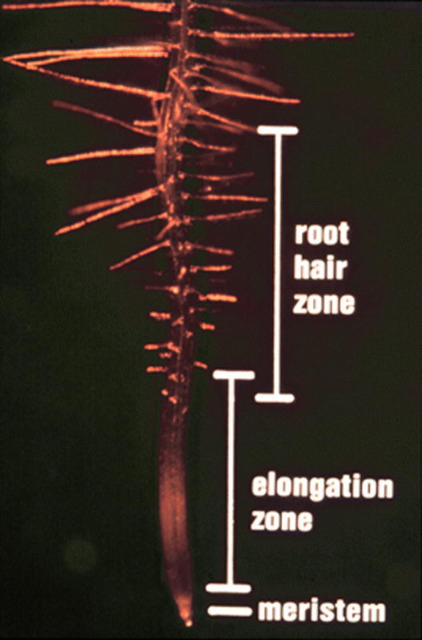
\includegraphics[height=0.35\textheight]{fig01/devepzones}
% 	\mycaption[Developmental zones of an Arabidopsis root.]{Developmental zones of an Arabidopsis root. Figure reproduced from \cite{griersonRH}.}
% 	\label{fig:RHP02}
% \end{figure}

%=========================================================